\chapter{Eletromiografia de Superfície - sEMG}
\section{Definição}
A eletromiografia de Superfície é o estudo relacionado às transformações elétricas das contrações musculares. É um exame indolor e não invasivo permitindo assim a execução com mobilidade dos movimentos musculares solicitados, podendo ser executada repetidas vezes sem causar um grande desconforto ao paciente, sendo rápida, barata, livre de radiação, não invasivo e de fácil compreensão, podendo ser utilizado na análise de um grupo ou um feixe muscular específico \cite{de2010eletromiografia}.

Um sinal sEMG é um sinal obtido na medição das tensões relacionados as correntes elétricas durante a contração muscular, fornecendo assim em um intervalo de tempo a média desta atividade neuromuscular\cite{reaz2006techniques}.

A sEMG caracteriza-se pela utilização de um dispositivo sobre a pele do paciente, o qual implica a detecção dos potenciais elétricos relativos às fibras musculares, ou seja é possível detectar quando um músculo é ativado e qual o movimento foi executado, e ainda relacionar o associação dos diferentes músculos envolvidos \cite{botelho2010avaliaccao}.

O sinal EMG é registrado normalmente por eletrodos de superfície, mas pode também ser utilizado eletrodos de agulha \cite{eftaxias2015detection}.

\section{Características do sinal}

Primeiramente temos a Unidade motora (MU - \textit{Motor Unit}), uma coleção de fibras musculares inervadas por um único neurônio motor alfa, sendo a menor unidade operacional de um músculo, podendo ser ativada pelo controle neural. A atividade muscular ocorre a ativação do neurônio alfa dentro da MU, produzindo tensão nas fibras musculares ao passo que ocorre a propagação do sinal ao longo das fibras, o músculo é relaxado quando o neurônio alfa para a atividade \cite{yousefi2014characterizing}.

O potencial de ação da unidade motora (\textit{motor unit potential} (MUP)) é a soma dos potenciais de ação das contrações musculares em uma unidade motora, as voltagens detectadas pelos eletrodos da sEMG, descrevem a soma de todas as UM ativas, ou seja a soma de todos os MUP \cite{yousefi2014characterizing}.

A figura ~\ref{UnidadeMotora}, representa um esquema simplificado da comunicação do neurônio com a unidade motora do músculo, o detalhamento dessa comunicação não é o objetivo deste trabalho.

\begin{figure}[!htb]
   \centering
    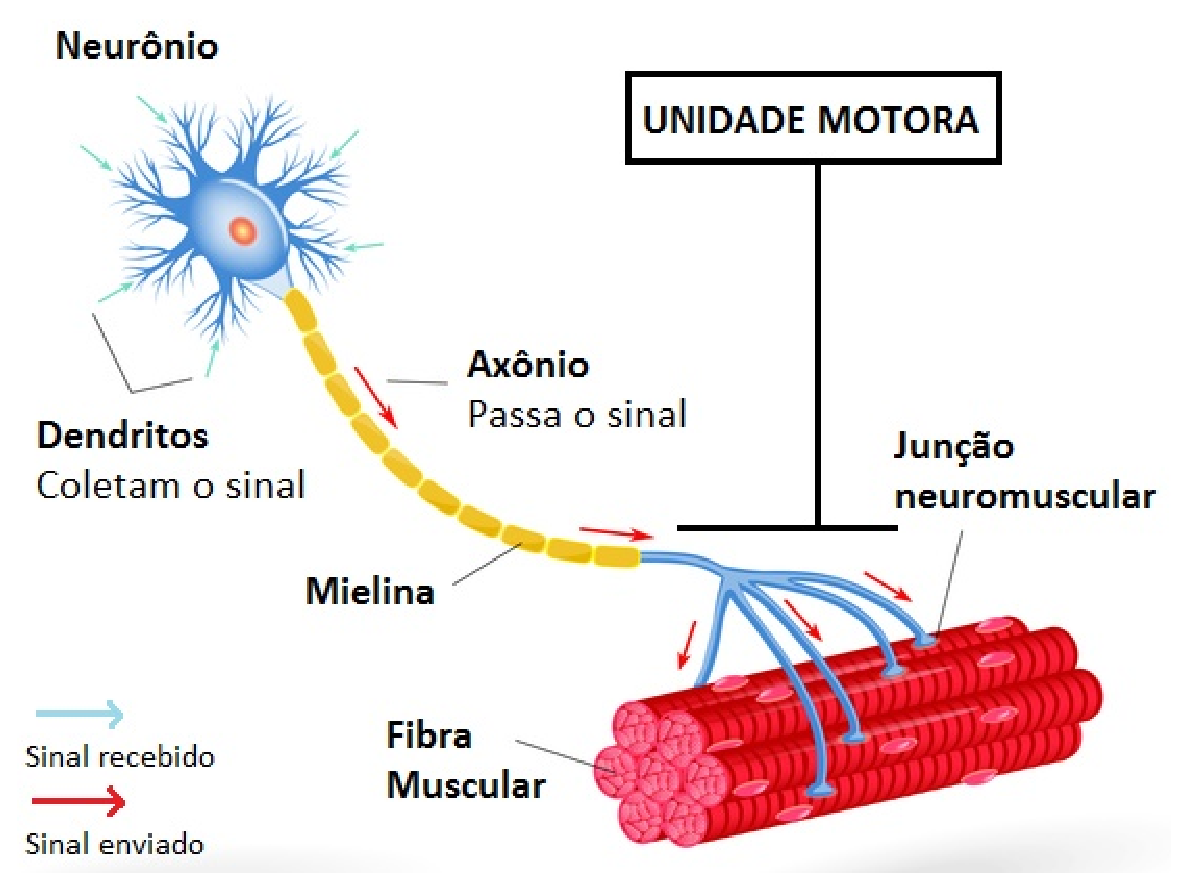
\includegraphics[width=0.8\textwidth]{figuras/motor-neuron.eps}
    \caption{Modelo de uma unidade motora.}
    \label{UnidadeMotora}
\end{figure}

A equação que descreve um sEMG é ~\ref{eq:EMGT}. Um sEMG é a medida ao longo do tempo da contração de um MUP m, de um total de N MUPs, a função n(t) representa possíveis ruídos encontrados na coleta, ambas as funções são parametrizadas pelo tempo \cite{yousefi2014characterizing}.

\begin{equation} \label{eq:EMGT}
    EMG_{t} =\sum_{m=1}^{N} MUPs_{m}(t)+n(t)
\end{equation}

Este tipo de sinal inevitavelmente encontra ruído do equipamento e de outras fontes biológicas presentes no corpo do indivíduo \cite{yousefi2014characterizing}.

Com relação a DP o tremor de repouso é o sintoma mais comum, possuindo uma frequência entre 4 e 6 Hz.
\cite{jankovic2008parkinson}

\section{Usos}
A sEMG é largamente utilizada por pelas diversas áreas científicas que estudam o movimento humano, como Médicos, Fisioterapeutas, Fonoaudiólogos e profissionais em Educação Física\cite{nascimento2012surface}.

\section{sEMG e machine learning}
A utilização de Aprendizado de máquinas em conjunto com sEMG para o auxílio na detecção de alguma doença, já é um tópico bem explorado possuindo diversas publicações relacionadas a esta área de estudo, na base de dados Capes a string de busca '(emg AND (Machine learning))' retornou 4.217 resultados, no \textit{ScienceDirect} a mesma \textit{string} retornou 2.396 no \textit{ieeexplore} 169.

Como observado na revisão acadêmica de \cite{yousefi2014characterizing}, os estudos relacionados a sEMG e machine learning são separados em  dois tipos de transtornos neuromusculares Miopatia e Neuropatia, onde Miopatia refere-se a um grupo de patologias que atingem diretamente o tecido muscular sem relação com disfunções do sistema nervoso. Já a Neuropatia, onde encontra-se a doença de Parkinson, é caracterizada por qualquer dano nos nervos envolvidos no controle muscular. Ambos os casos possuem diferenças e similaridades, em resumo segundo \cite{yousefi2014characterizing} as diversas técnicas de Aprendizado de máquinas sobre sEMG, pode-se catalogá-las em três etapas, análise, decomposição e classificação.

\subsection{Análise}
O pré-processamento ou análise dos dados é uma das partes mais importantes do processo de aprendizado, essa etapa consiste na etapa seguinte a coleta possuindo alguns objetivos como organizar os dados em conjuntos, tratar possíveis problemas com ruídos ou valores desconhecidos, também é comum utilizar esta etapa simplesmente aprender mais sobre os modelos plotando gráficos, ou ainda realizar tratamento nos dados como transformações lineares para um conjunto de dados mais simples de ser trabalhado. \cite{batista2003pre} A figura ~\ref{tremor_i_parkinson} representa o sinal EMG do tremor de intensão do grupo com a doença de Parkinson e  a figura ~\ref{tremor_intensao} corresponde ao grupo de controle, estes modelos foram coletados na fase de pré-processamento do projeto.


\begin{figure}[!htb]
   \centering
    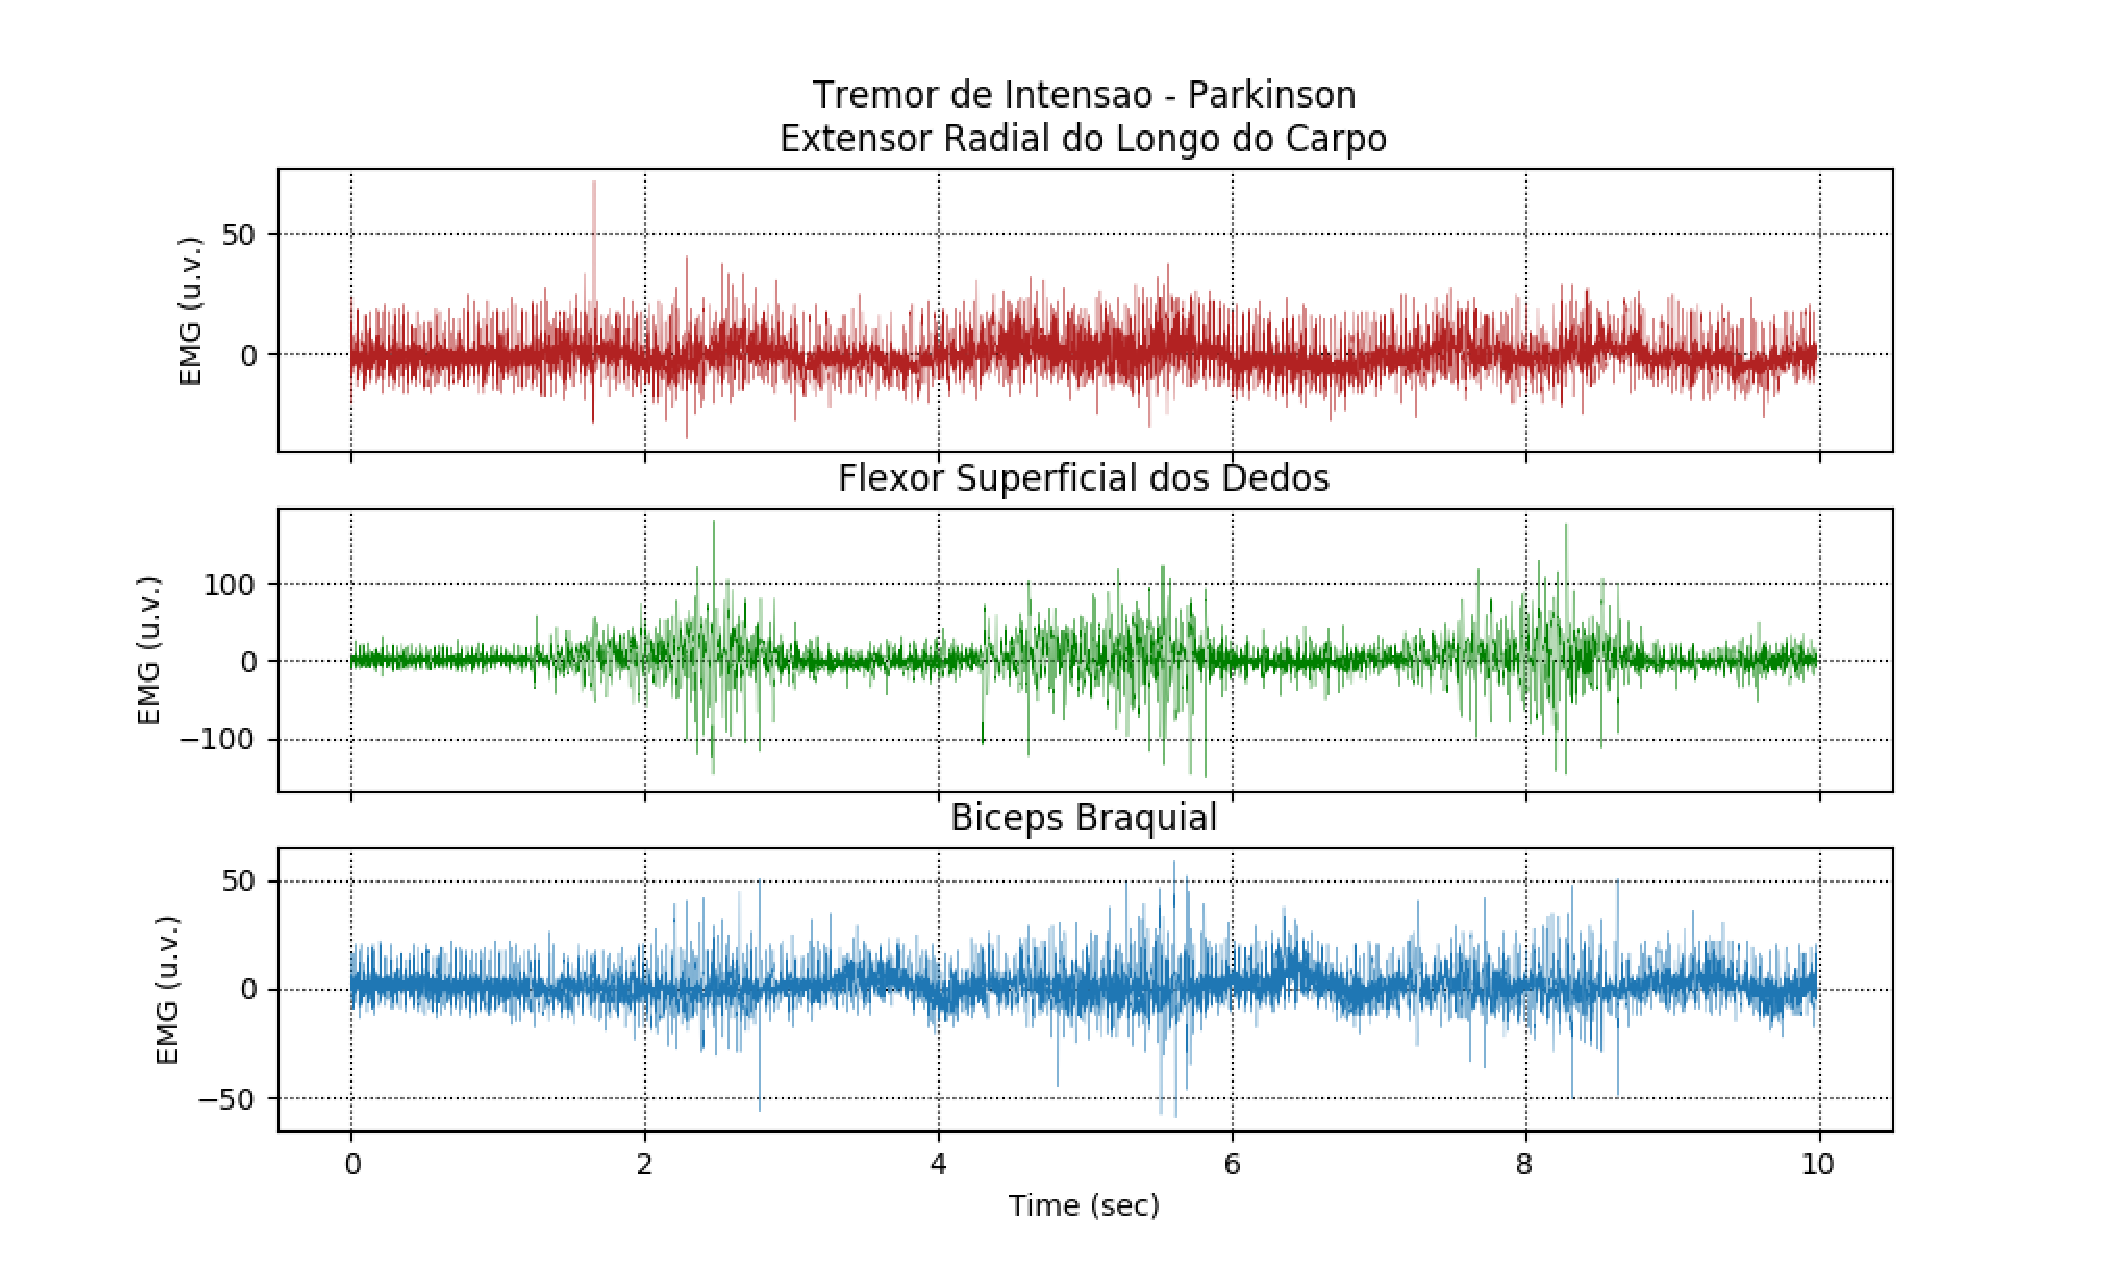
\includegraphics[width=1\textwidth]{figuras/tremor_i_parkinson.eps}
    \caption{PROVISSORIO!!!sEMG do tremor de intensão grupo com a Doença de Parkinson}
    \label{tremor_i_parkinson}
\end{figure}

\begin{figure}[!htb]
   \centering
    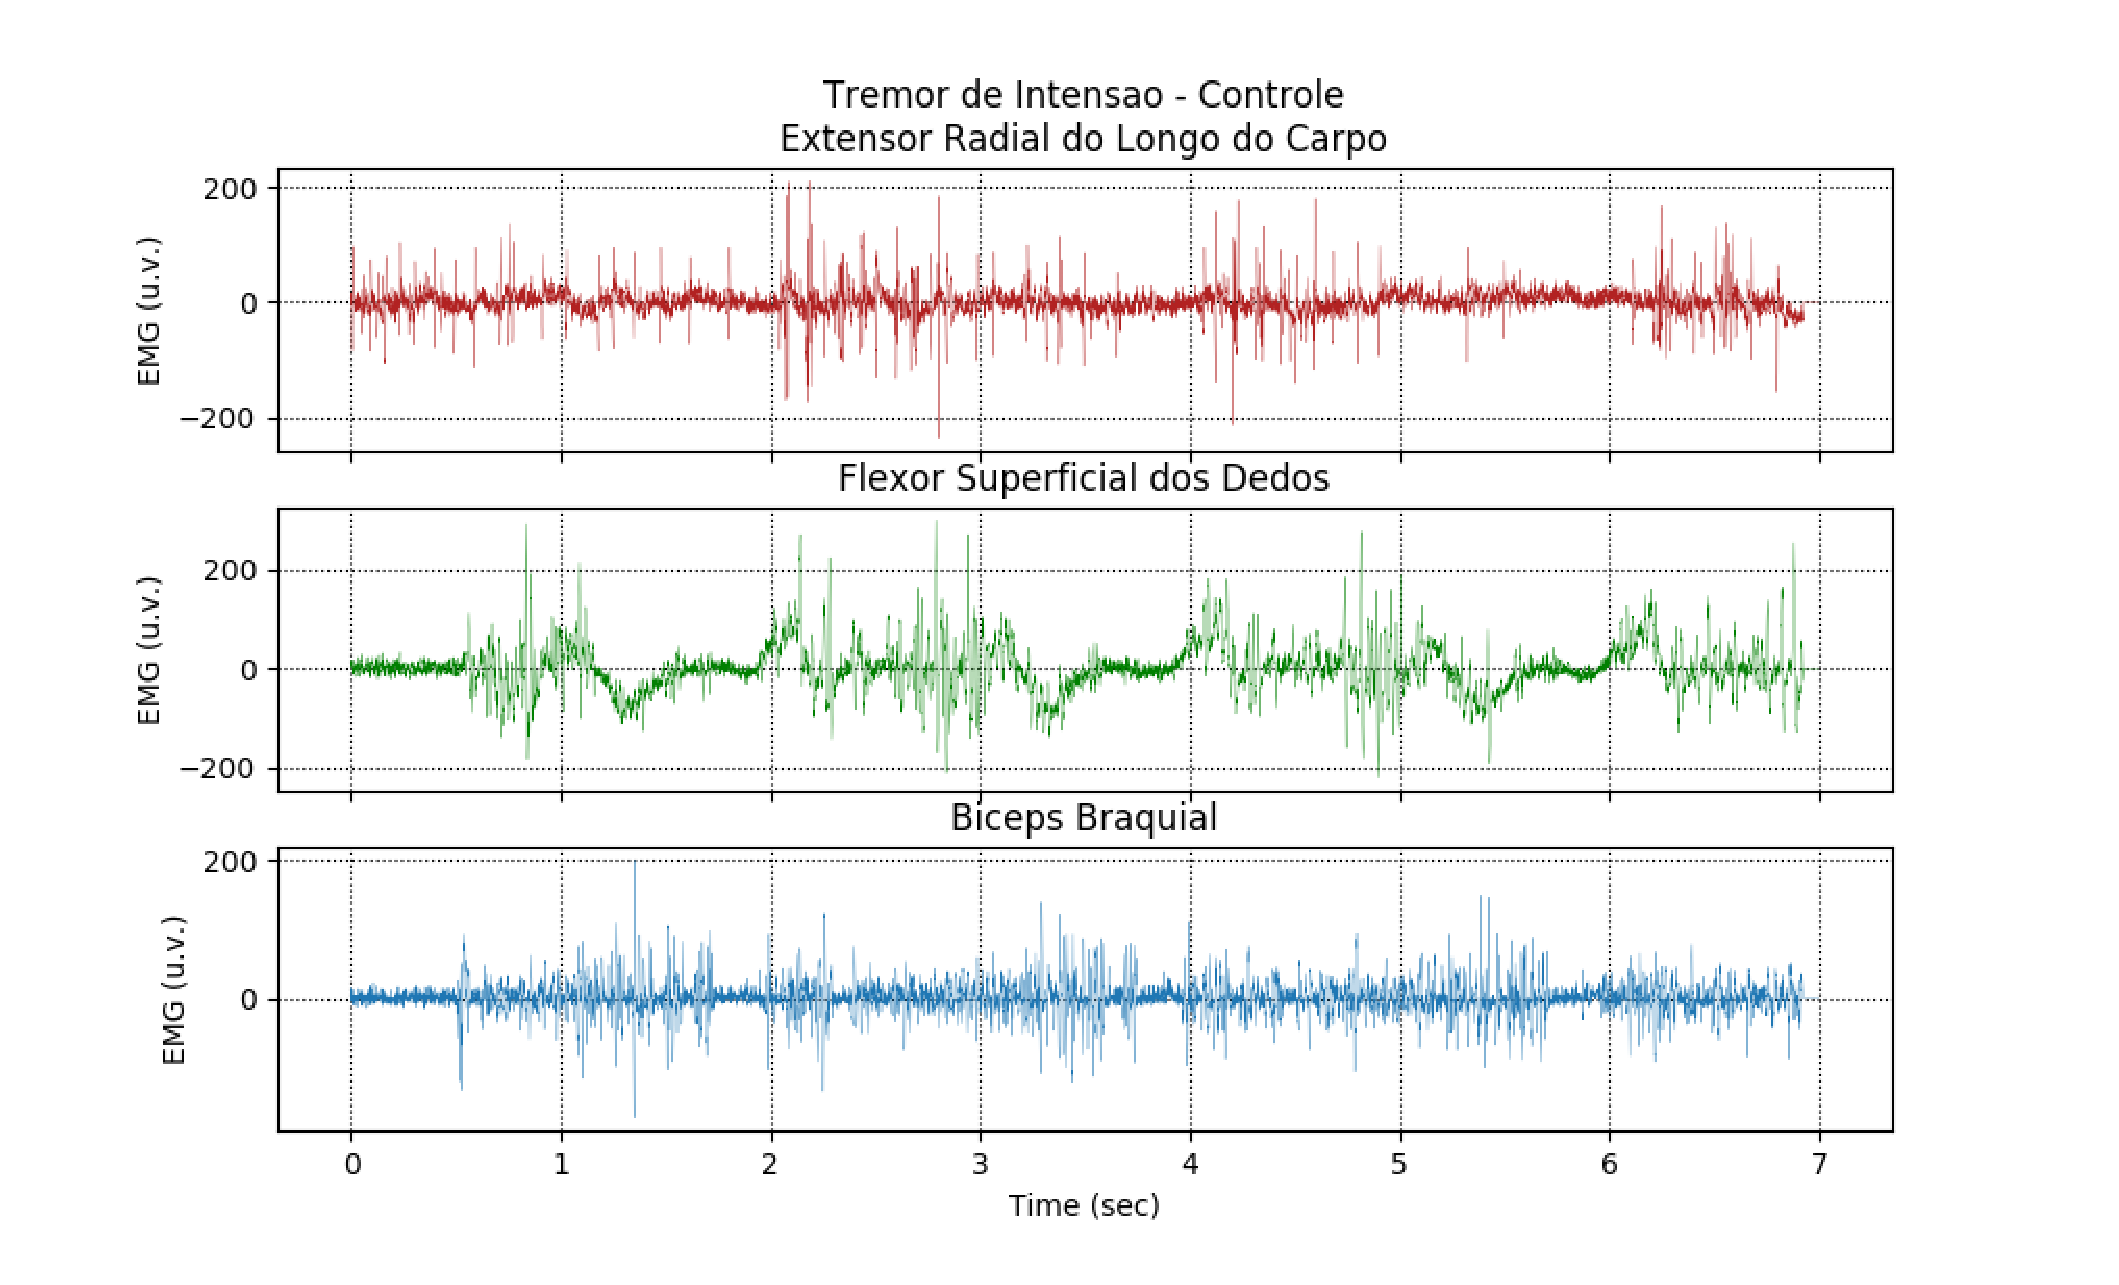
\includegraphics[width=1\textwidth]{figuras/tremor_intensao.eps}
    \caption{PROVISSORIO!!!sEMG do tremor de intensão grupo de controle}
    \label{tremor_intensao}
\end{figure}

\subsection{Decomposição}


